\documentclass{beamer}

\usepackage{../Research}

\newcommand{\F}{\mathcal F}
\newcommand{\curly}[1]{\left\{ #1 \right\}}

\title{VC-density in model theoretic structures}
\author{Anton Bobkov}
\date{June 3, 2015}


\begin{document}

\maketitle

\begin{frame}
	Suppose we have an (infinite) collection of sets $\F$. \\
	We define a shatter function $\pi_\F(n)$

	\begin{align*}
		\pi_\F(n) = \max \{ &\text {\# of atoms in boolean algebra generated by $S$} \\
		            &\mid S \subset \F \text{ with } |S| = n\}
	\end{align*}
\end{frame}

\begin{frame}
	Example: Let $\F$ consist of all discs on a plane.
	\begin{figure}[p]
    \centering
    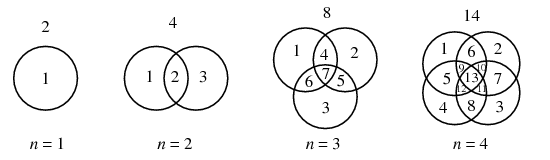
\includegraphics[scale=0.75]{circle.png}
	\end{figure}
	\begin{align*}
		\pi_\F(1) = 2 \ \ \  \pi_\F(2) = 4 \ \ \  \pi_\F(3) = 8  \ \ \ \pi_\F(4) = 14
	\end{align*}
	\begin{align*}
		\pi_\F(n) = n^2 - n + 2
	\end{align*}
\end{frame}

\begin{frame}
More examples: \\
	\begin{enumerate}
		\item Lines on a plane $\pi_\F(n) = n^2/2 + n/2 + 1$
		\item Disks on a plane	$\pi_\F(n) = n^2 - n + 2$
		\item Balls in $\R^3$  $\pi_\F(n) = n^3/3 - n^2 + 8n/3$
		\item Intervals on a line $\pi_\F(n) = 2n$
		\item Half-planes on a plane $\pi_\F(n) = n(n+1)/2 + 1$
		\item Finite subsets of $\N$ $\pi_\F(n) = 2^n$
		\item Polygons in a plane $\pi_\F(n) = 2^n$
	\end{enumerate}
\end{frame}

\begin{frame}
	\begin{Theorem} [Sauer-Shelah '72]
		Shatter function is either $2^n$ or bounded by a polynomial.
	\end{Theorem}
	\begin{Definition}
		Suppose growth of shatter function for $\F$ is polynomial.
		Let $r$ be the smallest real such that 
		\begin{align*}
			\pi_\F(n) = O(n^r)
		\end{align*}
		We define such $r$ to be the vc-density of $\F$, $\vc(\F)$.
		If shatter function grows exponentially, we let the vc-density to be infinite.
	\end{Definition}
\end{frame}

\begin{frame}
	\frametitle{Applications}
	\begin{itemize}
		\item NIP theories
		\item VC-Theorem in probability (Vapnik-Chervonenkis '71)
		\item Computational learning theory (PAC learning)
		\item Computational geometry
		\item Functional analysis (Bourgain-Fremlin-Talagrand theory)
		\item Abstract topological dynamics (tame dynamical systems)
	\end{itemize}
\end{frame}

\begin{frame}
	\frametitle{History}
	\begin{itemize}
		\item Vapnik-Chervonenkis '71 - introduce VC-dimension
		\item NIP theories (Shelah '71, '90)
		\item vc-density (Aschenbrenner, Dolich, Haskell, Macpherson, Starchenko '13)
	\end{itemize}
\end{frame}

\begin{frame}
	\frametitle{Model Theory}
	Model Theory studies definable sets in first-order structures.
	\begin{align*}
		(\Q, 0, 1, +, \cdot, \leq)
	\end{align*}
	\begin{align*}
		\phi(x) = \exists y \ y \cdot y = x
	\end{align*}
	In the structure above $\phi(x)$ defines a set of numbers that are a square.
\end{frame}

\begin{frame}
	\begin{align*}
		(\R, 0, 1, +, \cdot, \leq)
	\end{align*}
	\begin{align*}
		\phi(x) = \exists y \ y \cdot y = x
	\end{align*}
	In the structure above $\phi(x)$ defines the set $[0, \infty)$.
\end{frame}

\begin{frame}
	\begin{align*}
		(\R, 0, 1, +, \cdot, \leq)
	\end{align*}
	\begin{align*}
		\psi(x_1, x_2) = (x_1 \cdot x_1 + x_2 \cdot x_2 \leq 1.5) \wedge (x_1^2 \leq x_2)
	\end{align*}
	This defines a set in $\R^2$.
\end{frame}

\begin{frame}
	We work with families of uniformly definable sets.
	Fix a formula $\phi(x_1 \ldots x_n, y_1, \ldots y_m) = \phi(\vec x, \vec y)$.
	Plug in elements from the model for $y$ variables to get a family of definable sets in $M^n$.
	\begin{align*}
		\F^M_\phi = \curly{\phi(x_1, \ldots, x_n, a_1, \ldots a_n) \mid a_1, \ldots a_n \in M}
	\end{align*}
	Define $\vc^M(\phi)$ to be the vc-density of the family $\F^M_\phi$ \\
	Open Question: it is possible for $\vc^M(\phi)$ to be irrational?
\end{frame}

\begin{frame}
	\begin{align*}
		\phi(x_1, x_2, y_1, y_2, y_3) = (x_1 - y_1)^2 + (x_2 - y_2)^2 \leq y_3^2
	\end{align*}
	In structure $(\R, +, \cdot, \leq)$ given $a,b,r \in \R$ the formula $\phi(x_1, x_2, a, b, r)$ defines a disk in $\R^2$ with radius $r$ with center $(a,b)$.
	Thus $\F^\R_\phi$ is a collection of all disks in $\R^2$.
\end{frame}

\begin{frame}
	Shelah ('90) classified number of isomorphic classes for non-standard models.
	Important groups of structures included: stable, NIP, simple.
	A model $M$ is said to be NIP if all uniformly definable families in it have finite $\vc$-density.
	\begin{itemize}
		\item $(\C, 0, 1, +, \cdot)$ is stable (so both NIP and simple)
		\item $(\R, 0, 1, +, \cdot, \leq)$ is NIP and not stable
		\item $(\Q_p, 0, 1, +, \cdot, \mid)$ is NIP and not stable
		\item Random graph $(V, R)$ is simple and not stable.
		\item Pseudo-finite fields are simple and not stable.
		\item $(\Q, 0, 1, +, \cdot)$ is in neither of those categories.
	\end{itemize}
\end{frame}

\begin{frame}
	Given an NIP structure $M$ we define a vc-function of $n$ to be the largest $\vc$-density achieved by families of uniformly definable sets in $M^n$.
	\begin{align*}
		\vc^M(n) = max \curly{ \vc(\phi) \mid \phi(\vec x, \vec y) \text{ with } |\vec x| = n}
	\end{align*}
	Easy to show $\vc^M(n) \geq n \vc(1)$, $\vc(1) \geq 1$ \\
	Open question: Is $\vc^M(n) = n \vc^M(1)$? If not, is there a linear relationship?
\end{frame}

\begin{frame}
	Examples
	\begin{itemize}
		\item $(\R, 0, 1, +, \cdot, \leq)$ has $\vc(n) = n$ (true for all quasi o-minimal structures)
		\item $(\C, 0, 1, +, \cdot)$ has $\vc(n) = n$
		\item $(\Q_p, 0, 1, +, \cdot)$ has $\vc(n) \leq 2n - 1$
		\item ACVF has $\vc(n) \leq 2n$.
	\end{itemize}
\end{frame}

\begin{frame}
	\frametitle{vc-density in trees}
	Consider structure $(T, \leq)$ where elements of $T$ are vertices of a rooted tree and we say that $a \leq b$ if $a$ is below $b$ in the tree.
	\begin{itemize}
		\item Trees are NIP (Parigot '82)
		\item Trees are dp-minimal (Simon '11)
		\item Trees have $vc(n) = n$ (B. '13)
	\end{itemize}
\end{frame}

\begin{frame}
	$\tp(a)$, a type of an element $a$ is a set of all the formulas that that are true about $a$.\
	Parigot's observation: there is a natural way to split a tree into parts $A, B$ such that for $a \in A$ and $b \in B$ we have
	\begin{align*}
		\tp(a), \tp(b) \vdash \tp(ab)
	\end{align*}
	This allows us to decompose complex types into simple parts, which we can use to compute $\vc$-density.
\end{frame}

\begin{frame}
	\frametitle{Future work}
	\begin{itemize}
		\item $(\Q_p, 0, 1, +, \cdot, \mid)$
		\item Other partial orderings, lattices
		\item Other graph structures, in particular flat graphs
	\end{itemize}
\end{frame}

\end{document}

\begin{frame}
	\frametitle{vc-density in Shelah-Spencer graphs}
	Consider a random graph on $n$ vertices where the probability of the given two vertices having an edge is $n^{-\alpha}$.
	Shelah-Spencer graph is a limit of such graphs for $\alpha$ irrational in $(0,1)$.
	We view it in a language with a single binary relation.
	\begin{itemize}
		\item Shelah-Spencer graphs can be axiomatized (Shelah-Spencer '88)
		\item Shelah-Spencer graphs are stable (Baldwin-Shi '96, Baldwin-Shelah '97 )
	\end{itemize}

	We show that $\vc^V(1) = \infty$, so vc-function is infinite. However to any formula $\phi(\vec x, \vec y)$ we can prescribe a natural notion of dimension $\epsilon$, and we have
	\begin{align*}
		\vc^V(\phi) < \frac{|x|}{\epsilon}
	\end{align*}
	So even though vc-function is not well-behaved, there is still a linear structure on vc-density.
\end{frame}

\begin{frame}
	To a finite graph $A$ assign a dimension $\delta(A) = |V| - \alpha |E|$. $B/A$ is an extension. $\delta(B/A)$ is $\delta(A) = |V_B/V_A| - \alpha |E_B/E_A|$. $B/A$ is called minimal if its dimension is negative, but every subextension is positive. $(A_0, \ldots A_n)$ is a minimal chain if each $A_{i + 1}/A_i$ is minimal.
	Any 
\end{frame}

